\documentclass[10pt,letterpaper]{article}
\usepackage{elec3544_report}
\usepackage[T1]{fontenc}
\usepackage[utf8]{inputenc}
\usepackage{amsmath,amssymb,graphicx,booktabs,tabularx,nicefrac,xcolor}
\usepackage[hidelinks]{hyperref}
\usepackage{microtype,needspace}

\title{The Sunday Forecast: Predicting Next Week's Peak Steam Players\\with Baselines, Boosted Trees, and a Foundation Model}
\author{Group 18\\
{}Brown Destiny Sotonye (3036456475)\\
{}Tam Hoi Wing ([Student ID])\\
{}Soha Ali ([Student ID])}

\begin{document}
\maketitle

\begin{abstract}
We ask whether next week's peak player count for 24 Steam games can be predicted better than assuming the peak will not change, using only information public by Sunday 23:59 UTC. We build a weekly panel (312 game-weeks, August--November 2026) from SteamCharts histories, our own two-leg hourly recorder, and the Steam news API, with momentum, calendar, peer-group, and news features. Models are compared on chronological splits with the test weeks scored once; a final forecast for 9--15 November was sealed on GitHub before that week existed and scored against recorder data collected afterward. On the historical test, ridge regression beats the unchanged-peak baseline by 12\% (mean absolute error of log-growth 0.1263 vs.\ 0.1440, ratio 0.876) and a zero-shot foundation model (Chronos-2) barely beats it (0.973). On the sealed live week the edge does not survive (ratio 1.041): the week contained a 21$\times$ expansion surge we had named in writing, before it happened, as the model's known blind spot. We analyze the failure row by row and verify all peaks across three independent data legs.
\end{abstract}

\section{Introduction}
Steam publishes live concurrent-player counts for every game, and third-party archives make them historical. A game's weekly peak is commercially meaningful --- it drives server capacity, marketing timing, and chart position --- yet most weeks it barely moves, while a few weeks it multiplies on a release, sale, or expansion. This asymmetry defines our task: for 24 games followed weekly from August to November 2026, predict
\[
\text{log-growth} \;=\; \log(\text{next week's peak}) - \log(\text{this week's peak}),
\]
using only features known by Sunday 23:59 UTC, and beat the free baseline that predicts zero. Success is a mean absolute error (MAE) of log-growth below the baseline's, i.e.\ an error ratio under 1, on a chronological test scored once --- and, unusually for a course project, on a \emph{sealed forecast} committed before the target week existed and scored against data collected afterward. Our contributions: (i) a leakage-disciplined weekly panel with momentum, calendar, peer, and news features; (ii) a frozen five-model ladder including a zero-shot time-series foundation model \citep{ansari2024chronos}; (iii) a pre-registered live evaluation whose failure mode we named in writing five days before it occurred.

\section{Data and Preprocessing}
\textbf{Sources.} Three primary sources, all public \citep{steamcharts,steamwebapi}: (1) SteamCharts per-game histories (\texttt{chart-data.json}) for 24 games, downloaded 4, 8, and 16 November 2026; (2) our own hourly recorder hitting the Steam API's \texttt{GetNumberOfCurrentPlayers}, run on two independent legs (a macOS \texttt{launchd} job and GitHub Actions) from 5 November onward, $\sim$5{,}500 rows per leg; (3) the Steam news API (\texttt{GetNewsForApp}) for update detection. Figure~\ref{fig:cutoff} shows the forecasting setup on one recognizable series.

\begin{figure}[t]
\centering
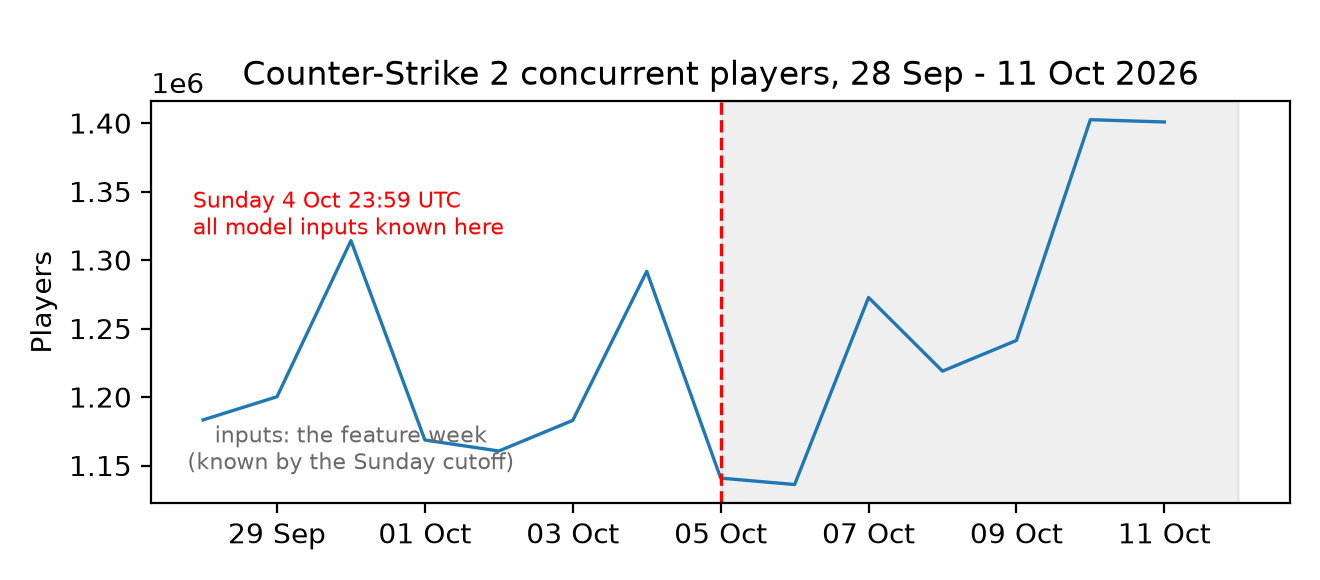
\includegraphics[width=\linewidth]{figures/fig_cutoff.png}
\caption{Counter-Strike 2 concurrent players around the week of 28 September 2026. Features may use only observations left of the Sunday cutoff; the shaded week is the prediction target.}
\label{fig:cutoff}
\end{figure}

\textbf{Panel.} Weeks run Monday 00:00 to Sunday 23:59 UTC. The panel holds 312 game-weeks (24 games $\times$ 13 weeks, 10 August--2 November). SteamCharts resolution varies: monthly before August, daily 9 August--6 October, hourly afterward; a \texttt{resolution} column records this, and early-week peaks are daily maxima, not true hourly peaks --- a stated limitation. Isolated zero player counts (API artifacts) are dropped from peaks and means but kept in an \texttt{n\_zeros} count. From the series we compute per game-week: peak, mean, sample counts, momentum (week-over-week growth, trailing four-week growth/median/MAD with a missing-window flag), calendar (weekend days, sale this/next week, holiday count, each with a publicly announced date), peer momentum (leave-one-out group median of week-over-week growth; five genre groups of 4--6 games), and news (post count, days since last post, a \texttt{major\_update} heuristic from title patterns such as numbered patches and named content drops, flagged on 53 of 312 rows). Peaks and means enter models log-scaled so all features are size-free.

\textbf{Refused sources, documented.} Twitch was omitted because the Helix API reports streams only live --- no historical hours-watched series exists to train on; SullyGnome has no API and was hand-read for at most one case illustration. Steam review velocity was probed on 5 November: the \texttt{appreviews} JSON endpoint returned an unconditional 302 redirect, and SteamSpy exposes only cumulative counts. These refusals, with verbatim evidence, are in the repository's session log \citep{group18repo}.

\section{Methodology}
\textbf{Target, metric, baseline.} Models predict log-growth; the error is its MAE, reported alongside the ratio to the unchanged-peak baseline (predict 0). Most weekly peaks move little, so the baseline is strong and free; any model must beat it to justify itself. Training $R^2$ on raw counts is not reported: game size dominates it, so even useless forecasts score well. We also define a \emph{surge}: next peak $\geq 1.5\times$ this peak \emph{and} at least two robust deviations above the trailing four-week median. Surges are rare --- 5 of 192 training rows (2.6\%, Figure~\ref{fig:surge}) --- so the growth error carries the evaluation and surges are studied as cases.

\begin{figure}[t]
\centering
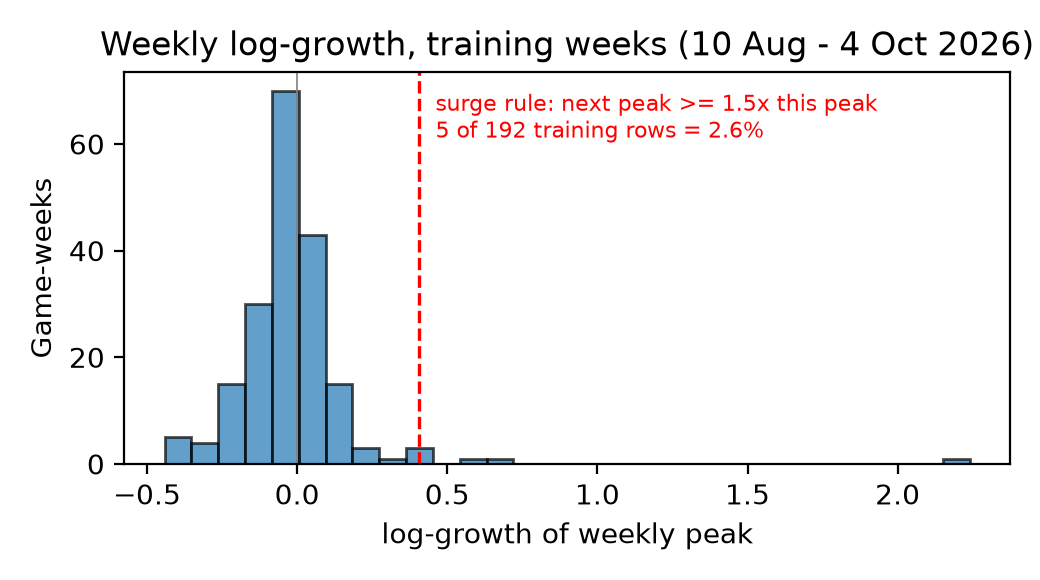
\includegraphics[width=0.8\linewidth]{figures/fig_surge_hist.png}
\caption{Training-week log-growth (192 game-weeks) with the surge threshold. The right tail --- not the center --- is where forecasts fail.}
\label{fig:surge}
\end{figure}

\textbf{Model ladder.} Five models, one target, one split, one metric. (1) \emph{Unchanged peak}: predict 0. (2) \emph{Weekday pattern}: predict next peak as the game's average historical peak --- a sanity check that calendar memory alone fails. (3) \emph{Ridge regression} on standardized features ($\alpha=1.0$; normal equations, no library model): the interpretable regularized linear. (4) \emph{Shallow XGBoost} \citep{chen2016xgboost} (depth 3, 100 trees, learning rate 0.1, seed 42): the nonlinear learner. (5) \emph{Chronos-2 small} \citep{ansari2024chronos}, zero-shot: weekly-peak context from 10 August through each row's own week (Sunday cutoff respected), one-step median forecast, player history only --- the course's foundation-model arm. The ladder is ordered so each rung answers a question the previous cannot: does regularization help, do nonlinearity and interactions help, does a large pretrained model transfer zero-shot?

\section{Experiments and Reproducibility}
\subsection{Experimental Protocol}
Splits are chronological, never random: a random split would let a model learn a game's later weeks and ``predict'' its earlier ones. Training: eight weeks starting 10 August (192 rows). Validation (model selection): 5--18 October (48 rows). Historical test: 19 October--1 November (48 rows), \emph{scored once} on 7 November with the ladder frozen; the second test week's outcomes (2--8 November) were 79--81 of 168 hourly samples complete at scoring, a stated limitation. Leakage controls: every feature for week $t$ uses timestamps inside $t$ or earlier; the live forecast for 9--15 November was emitted 8 November 15:59:30 UTC, committed to GitHub before the week began, and never edited. For the live forecast only, ridge was refit on all 288 labeled rows (standard post-evaluation practice; the test weeks precede the forecast week, so no leakage) --- the 0.876 test score belongs to the train-only fit and stands untouched. The live week was scored once, 16 November, against merged recorder data with zero-counts dropped.

\subsection{Data and Code for Reproduction}
Repository: \url{https://github.com/destiny-brown/Steam-Analysis}, commit \texttt{6e576b2} \citep{group18repo}. Pipeline order: \texttt{collect/download\_steamcharts.py --refresh} $\rightarrow$ \texttt{model/build\_week\_panel.py} $\rightarrow$ \texttt{model/train.py} (writes \texttt{validation.csv}, \texttt{test.csv}, \texttt{ablation.csv}) $\rightarrow$ \texttt{model/run\_chronos.py} $\rightarrow$ \texttt{model/forecast.py} (sealed forecast) $\rightarrow$ \texttt{model/score\_live\_week.py} (writes \texttt{live\_week.csv}). Every number in this report is copied from those CSVs; the dated session log (\texttt{decisions.md}) records each decision when made.

\subsection{Computing Platform and Environment}
Personal MacBook (Apple M1), macOS, CPU only. Python 3.14.7; NumPy 2.5.4 \citep{harris2020numpy}, pandas 3.1.1 \citep{mckinney2010pandas}, matplotlib 3.11.2 \citep{hunter2007matplotlib}, XGBoost 3.4.1 \citep{chen2016xgboost}, PyTorch 2.15.0, chronos-forecasting 2.3.2 (\texttt{autogluon/chronos-2-small}, accessed 7 November 2026) \citep{ansari2024chronos}. Panel build under a minute; the classical ladder fits in seconds; Chronos-2 zero-shot inference for 48 rows ran on CPU. Data collection used the two recorder legs above at hourly cadence.

\section{Results and Discussion}
\subsection{Historical evaluation}
Table~\ref{tab:ladder} is the frozen ladder. Two findings survive contact with the test weeks. First, \emph{regularization beats capacity}: ridge generalizes (train 0.112, test 0.126) where XGBoost overfits (train 0.044, test 0.132), so the simplest real model wins the test. Second, \emph{the foundation model's zero-shot edge is thin}: Chronos-2 beats the baseline by under 3\% with no features at all --- impressive transfer, but far behind a ridge on hand-built features, an informative negative result for the foundation-model hypothesis at this data scale. The weekday-pattern sanity check fails catastrophically (ratio 2.291), confirming the target is not a memory problem. The ablation (Table~\ref{tab:ablation}) shows every feature family contributes on test: removing calendar or peer columns costs XGBoost most of its edge. Peer momentum alone is descriptive, not predictive: games move with their group in the same week 65.5\% of the time, but the group median predicts next week's direction only 54.8\% of the time --- below always guessing ``down'' (62.5\%) --- with RPGs the only strong group. Calendar flags show small, directionally sensible associations (sale weeks mean growth $-0.011$ vs.\ $-0.045$ without), descriptive only on eight training weeks.

\begin{table}[t]
\centering\small
\caption{Model ladder: MAE of log-growth (lower is better) and test ratio to the unchanged-peak baseline. Chronos-2 is zero-shot (no fit), evaluated on test only.}
\label{tab:ladder}
\begin{tabular}{lcccc}
\toprule
Model & Train MAE & Val MAE & Test MAE & Test ratio \\
\midrule
Unchanged peak (baseline) & 0.1141 & 0.0895 & 0.1440 & 1.000 \\
Weekday pattern & 0.1705 & 0.2255 & 0.3300 & 2.291 \\
\textbf{Ridge} & 0.1117 & 0.0980 & \textbf{0.1263} & \textbf{0.876} \\
Shallow XGBoost & 0.0442 & 0.1091 & 0.1319 & 0.916 \\
Chronos-2 small (zero-shot) & --- & --- & 0.1401 & 0.973 \\
\bottomrule
\end{tabular}
\end{table}

\begin{table}[t]
\centering\small
\caption{XGBoost ablation on the one-touch test weeks.}
\label{tab:ablation}
\begin{tabular}{lcc}
\toprule
Features & Test MAE & Ratio \\
\midrule
Full & 0.1319 & 0.916 \\
Without calendar & 0.1413 & 0.981 \\
Without peer momentum & 0.1424 & 0.988 \\
Without major-update flags & 0.1334 & 0.926 \\
\bottomrule
\end{tabular}
\end{table}

\begin{figure}[t]
\centering
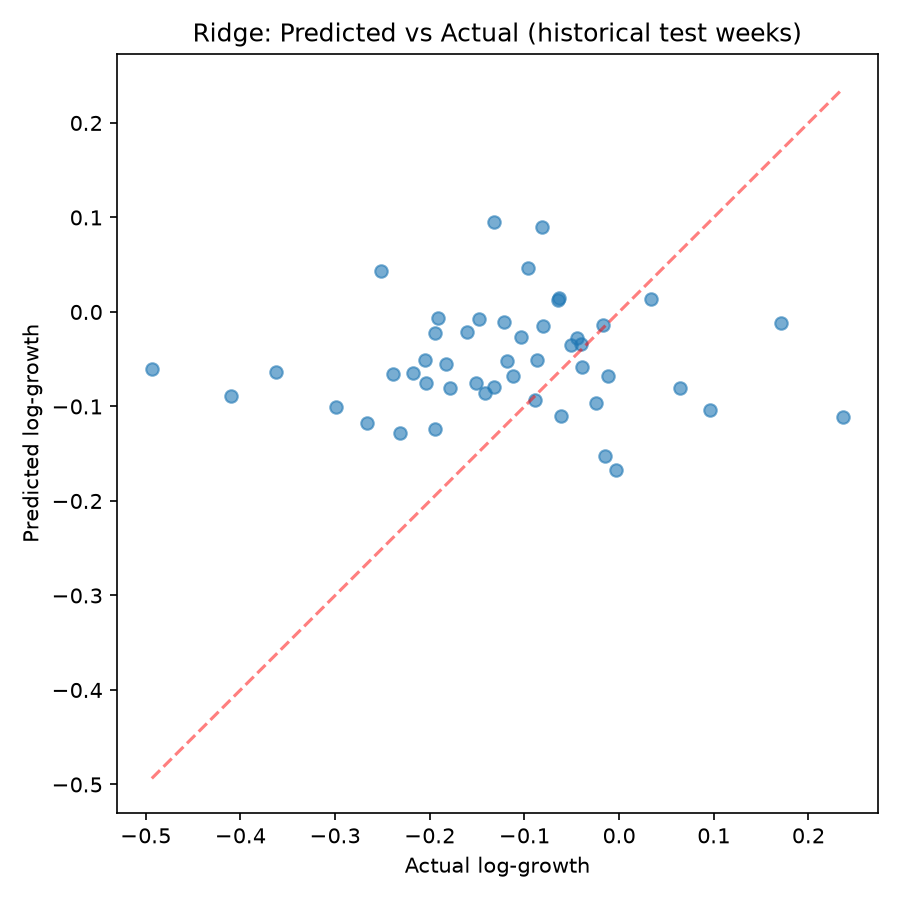
\includegraphics[width=0.62\linewidth]{figures/pred_vs_actual_test_ridge.png}
\caption{Ridge, the chosen model, on the one-touch historical test weeks (48 rows). The cloud tracks the perfect-prediction line in the center; errors concentrate in the same right tail as Figure~\ref{fig:surge}.}
\label{fig:testridge}
\end{figure}

\begin{figure}[t]
\centering
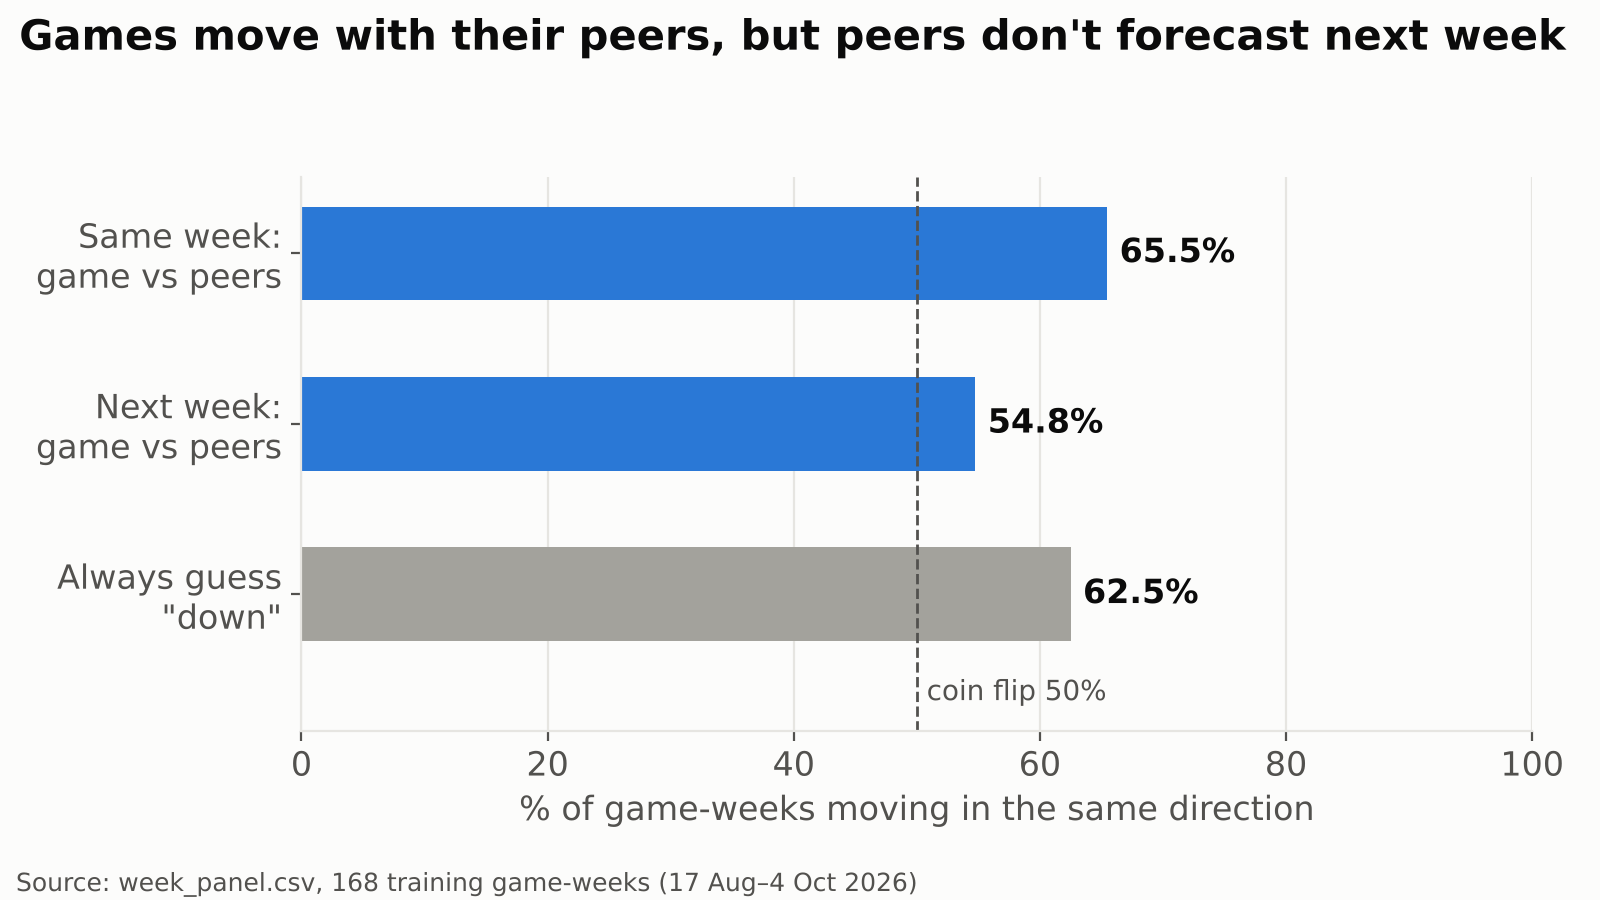
\includegraphics[width=0.62\linewidth]{figures/soha_peer_agreement.png}
\caption{Direction agreement with the peer-group median: clearly descriptive in the same week, no better than guessing ``down'' for the next.}
\label{fig:peer}
\end{figure}

Two case studies illustrate the error structure. HELLDIVERS 2 (week of 19 October): own peak up 65\% week-over-week while peers drifted down; next week the peak fell 39\% --- peers and Chronos-2 both had the direction, neither the size (baseline error 0.494, three times the pooled test error). The calendar case (week of 19--25 October, Cooking Fest ended, Next Fest running, a Hong Kong holiday known Sunday) shows the feature vector as seen at prediction time; such weeks sit near the distribution's center, where the model is reliable.

\subsection{The sealed live week}
The forecast for 9--15 November (all 24 games predicted down, $-0.03$ to $-0.18$) was sealed on GitHub on 8 November and scored on 16 November against data that did not exist at seal time. Table~\ref{tab:live} and Figure~\ref{fig:live} carry the result: \textbf{the edge did not survive} (MAE 0.2281 vs.\ baseline 0.2190, ratio 1.041). The anatomy matters more than the number. Path of Exile's \emph{Covens of Umbra} expansion launched Friday 13 November; its peak went from 7.2k to 151.5k (log-growth $+3.05$, $\sim$21$\times$), and this single row contributes over half the total model error. Our seal-night log entry --- dated five days earlier --- names this exact event as ``the known wildcard, invisible to Sunday features.'' Marvel Rivals also surged ($+0.54$, a 1.7$\times$ surge by our own rule). Elsewhere the model behaved: it beat the baseline on 11 of 24 games, catching every large decline (HELLDIVERS 2, Rust, Lost Ark, Valheim), and lost predictably on flat games, where ``predict nothing'' is structurally unbeatable, and on seven modest rises against its down-bias. At a 2.6\% surge rate per game-week, a 24-game week had a $\sim$47\% chance of containing at least one surge; the draw was nearly a coin flip. Verification used three independent legs: the two recorders' peaks agree within 10\% on every game, and a post-week SteamCharts re-download agrees within 2.4\% on 23 of 24 games --- including both surges (Path of Exile 151{,}488 vs.\ 151{,}348) --- so the surges are real, not instrumentation error. The one exception (Team Fortress 2, 12.5\%) leaves the headline unchanged (ratio 1.041 either way).

\begin{table}[t]
\centering\small
\caption{The two evaluations, side by side. The historical edge is real; the sealed live draw contained the surge class the project documented as unpredictable.}
\label{tab:live}
\begin{tabular}{lccc}
\toprule
Evaluation & Model MAE & Baseline MAE & Ratio \\
\midrule
Historical test (48 game-weeks) & 0.1263 & 0.1440 & \textbf{0.876} \\
Sealed live week (24 game-weeks) & 0.2281 & 0.2190 & \textbf{1.041} \\
\bottomrule
\end{tabular}
\end{table}

\begin{figure}[t]
\centering
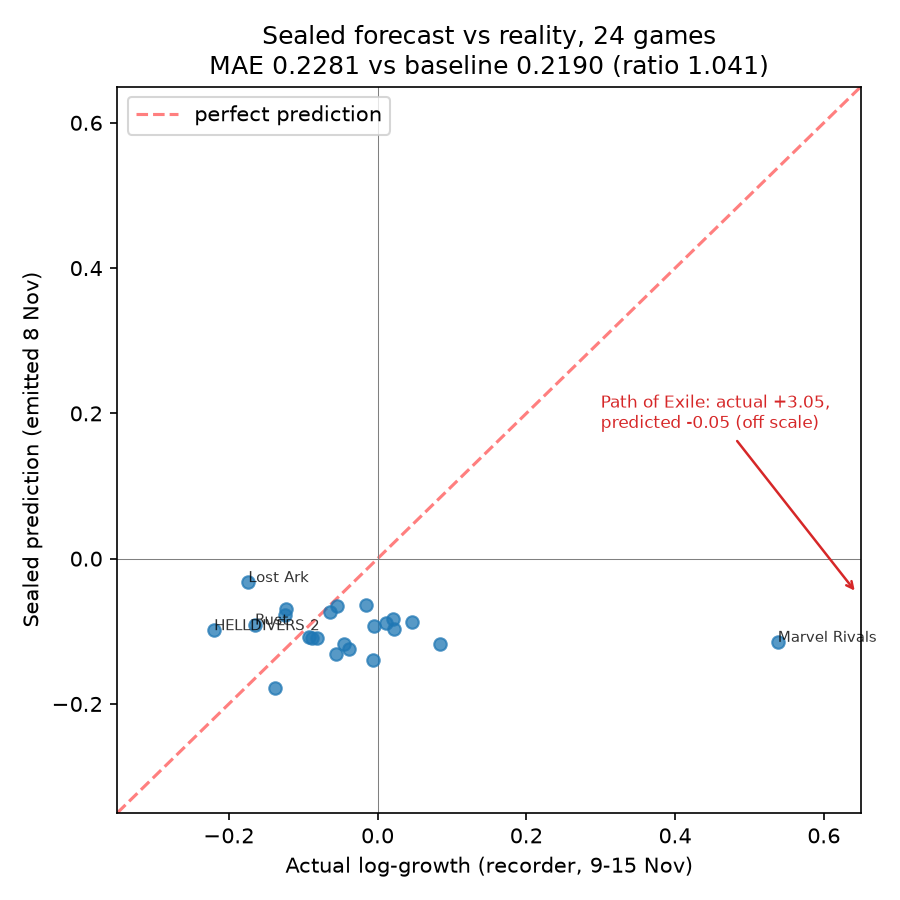
\includegraphics[width=0.72\linewidth]{figures/live_week_pred_vs_actual.png}
\caption{Sealed predictions vs.\ recorder reality, 9--15 November. The labeled upper-left outlier is Path of Exile's expansion week --- named in the sealed log before it happened.}
\label{fig:live}
\end{figure}

\textbf{Limitations.} Twelve usable weeks and 24 games; 48 rows per split, so single rows move ratios. Early weeks are daily samples, not true hourly peaks. The second historical test week's outcomes were incomplete at scoring. The live model is a refit, not the exact tested object. Momentum features derive from one series and correlate. Peer groups are hand-assigned. Nothing here shows a sale, post, or peer \emph{caused} a surge.

\section{Conclusion}
Can momentum, calendar, peer, and news features beat the unchanged-peak baseline? \emph{On held-out history, yes} --- ridge's 12\% edge with every feature family contributing on ablation. \emph{Does the edge survive a sealed forecast? Not this week} --- one draw containing a 21$\times$ surge we had identified, in advance and in writing, as the model's blind spot. The strongest supported findings: weekly peak growth is predictable in its center and not in its tail; regularized linear models on disciplined features currently beat both boosted trees and zero-shot foundation models at this scale; and pre-registered evaluation turns a losing week into evidence rather than embarrassment. The clearest next step follows directly from the miss: expansion and release dates are public \emph{calendar} information (Path of Exile's was announced long before 8 November), so a ``known future content'' feature --- not news about the present week --- is the obvious addition. Beyond that: more seasons of data, quantile rather than point forecasts, and a surge-class classifier.

\section*{Author Contributions}
\begin{center}
\small
\renewcommand{\arraystretch}{1.3}
\begin{tabularx}{\linewidth}{@{}p{0.95in}XX@{}}
\toprule
\textbf{Member name} & \textbf{Specific contributions} & \textbf{Evidence or output} \\
\midrule
{}Brown Destiny Sotonye & Two-leg hourly recorder (launchd + GitHub Actions), SteamCharts pipeline, weekly panel, five-model ladder and one-touch evaluation, ablation, Chronos-2 run, sealed forecast and live-week scoring, repository and session log & \texttt{collect/}, \texttt{model/}, \texttt{data/}, \texttt{decisions.md}; sealed forecast commit \texttt{4eeeebe}, scoring commit \texttt{6e576b2} \\
Tam Hoi Wing (Sienna) & Sale/holiday calendar research with announced dates, calendar features and comparison, data-quality section, calendar case study, calendar slides, hand-checked three SteamCharts pages & \texttt{analysis/calendar*}, \texttt{report/02\_data\_and\_calendar.md}, \texttt{report/slides\_sienna.md} \\
Soha Ali & Peer-group taxonomy (five groups), peer momentum feature and analysis, model-comparison and ablation write-up with figures, HELLDIVERS 2 case study, peer slides, hand-checked five baseline errors and the sealed file's names/timestamp & \texttt{analysis/peers*}, \texttt{report/01\_question\_and\_peers.md}, \texttt{report/slides\_soha.md}, \texttt{report/figures/} \\
\bottomrule
\end{tabularx}
\end{center}

\section*{AI Tool Use}
We used an AI coding assistant (Cursor) for code drafting, debugging, documentation wording, and report assembly. All AI outputs were verified by running the code against real data, cross-checking every reported number against the committed CSVs and the dated session log, and requiring each claim to trace to a repository artifact. Model selection, the evaluation protocol, the freeze discipline, and the seal/score decisions were made by the group. Every member can explain and defend the submitted work.

\Needspace{12\baselineskip}
{\small
\bibliographystyle{plainnat}
\bibliography{references}
}

\clearpage
\section*{Supplementary Materials}
Supplementary artifacts in the repository \citep{group18repo}: validation diagnostics (\texttt{pred\_vs\_actual.png}, \texttt{residuals.png}); the model-ladder bar chart (\texttt{report/figures/soha\_model\_ladder.png}); the full 24-row live-week scoring table with per-leg peaks (\texttt{model/results/live\_week.csv}); Chronos-2 per-row forecasts (\texttt{model/results/chronos\_note.txt}); recorder health logs for both legs (\texttt{data/live/collector\_runs.csv}, \texttt{data/live/cloud/}); the sealed forecast file itself (\texttt{data/live/forecast\_2026-11-09.csv}, emitted 8 November 2026 15:59:30 UTC); and the dated session log (\texttt{decisions.md}) from which this report's method section is drawn.

\end{document}
